\chapter{Introduction}
 \section{Motivation}


DBMSs are widely used in many fields and find application in many companies as they provide relatively easy way of performing various common operations on data, such as insertion, deletion and update, and at the same time they hide the internal complexity of such  system. More precisely, DBMS is a software that is designed to allow the creation, querying and update of databases [2,3]. The main role of a DBMS is to store and manipulate data efficiently and consistently. Figure 1.1 shows in a high level the structure of modern DBMSs. Additionally, Structured Query language  known as SQL is a standardised programming language for managing relational databases [1]. By having such standards, it can be provided easily a common interface for all DBMSs in order to manipulate and retrieve data from any given database without worrying about the internal implementation. 
 
The aim of this project is to evaluate five systems such as MySQL, IBM DB2, Microsoft SQL Server, PostgreSQL and Oracle Database in order to identify if they interpret the SQL standards in exactly the same way. 

 \begin{figure} 
      \centering
      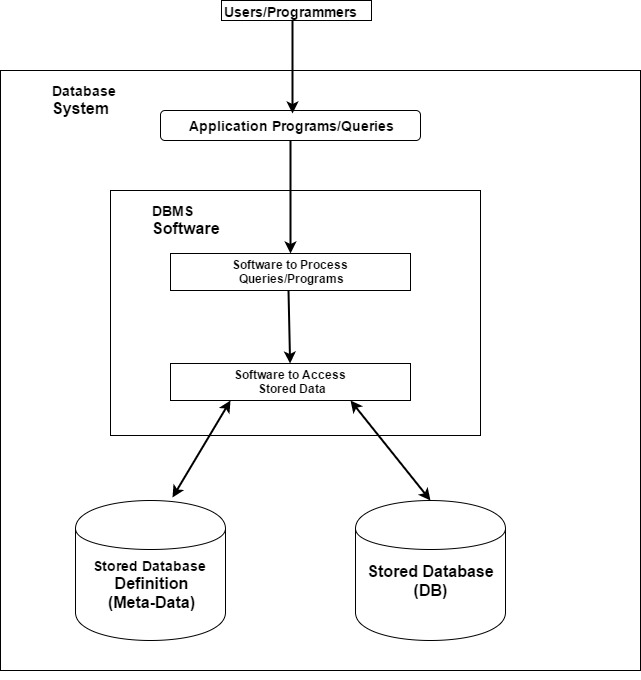
\includegraphics[width=\textwidth]{Images/db_architecture}
      \caption{DBS architecture}
      \label{fig:counting-methods}
    \end{figure}

As it was mentioned all current DBMSs currently support the SQL standards, meaning that there is a common language, namely SQL, that is used by all systems to access, manipulate and retrieve data. Nevertheless some aspects of the standards are not well defined which make the process of interpret and implement it a difficult task and as a results, companies implement the SQL standards in a different manner. As a consequence programs that are written in SQL are partially portable among different DBMS.  



\begin{table}[h]
\centering
\caption{My caption}
\label{my-label}
\begin{tabular}{lll}
\multicolumn{3}{l}{\textbf{Is it a bug?}}                                                                               \\
                                       & \multicolumn{1}{c}{\textbf{Y}}           & \multicolumn{1}{c}{\textbf{N}}      \\ \cline{2-3} 
\multicolumn{1}{l|}{\textbf{Bugs}}     & \multicolumn{1}{l|}{True Positive (TP)}  & \multicolumn{1}{l|}{False positive} \\ \cline{2-3} 
\multicolumn{1}{l|}{\textbf{Reported}} & \multicolumn{1}{l|}{False Negative (FN)} & \multicolumn{1}{l|}{True Negative}  \\ \cline{2-3} 
                                       &                                          &                                    
\end{tabular}
\end{table}


\begin{math}
\frac{2}{3}
\end{math}